\documentclass{article}
\usepackage[utf8]{vietnam}
\newif\ifanswers
\answerstrue % comment out to hide answers

\usepackage[compact]{titlesec}
\usepackage{fancyhdr} % Required for custom headers
\usepackage{lastpage} % Required to determine the last page for the footer
\usepackage{extramarks} % Required for headers and footers
\usepackage[usenames,dvipsnames]{color} % Required for custom colors
\usepackage{graphicx} % Required to insert images
\usepackage{listings} % Required for insertion of code
\usepackage{courier} % Required for the courier font
\usepackage{lipsum} % Used for inserting dummy 'Lorem ipsum' text into the template
\usepackage{enumerate}
\usepackage{enumitem}
\usepackage{subfigure}
\usepackage{booktabs}
\usepackage{amsmath, amsthm, amssymb}
\usepackage{caption}
\usepackage{hyperref}
\captionsetup[table]{skip=4pt}
\usepackage{framed}
\usepackage{bm}
\usepackage{minted}

\usepackage{tikz}
\usetikzlibrary{positioning,patterns,fit}
\usepackage{listings}
\usepackage{xcolor}

% Margins
\topmargin=-0.45in
\evensidemargin=0in
\oddsidemargin=0in
\textwidth=6.5in
\textheight=9.0in
\headsep=0.25in

\linespread{1.1} % Line spacing

% Set up the header and footer
\pagestyle{fancy}
\rhead{\hmwkAuthorName} % Top left header
\lhead{\hmwkClass: \hmwkTitle} % Top center head
\lfoot{\lastxmark} % Bottom left footer
\cfoot{} % Bottom center footer
\rfoot{Page\ \thepage\ of\ \protect\pageref{LastPage}} % Bottom right footer
\renewcommand\headrulewidth{0.4pt} % Size of the header rule
\renewcommand\footrulewidth{0.4pt} % Size of the footer rule

\setlength\parindent{0pt} % Removes all indentation from paragraphs

\newenvironment{answer}{
    % Uncomment this if using the template to write out your solutions.
    {\bf Answer:} \sf \begingroup\color{black}
}{\endgroup}% 
%----------------------------------------------------------------------------------------
%	CODE INCLUSION CONFIGURATION
%----------------------------------------------------------------------------------------

\definecolor{MyDarkGreen}{rgb}{0.0,0.4,0.0} % This is the color used for comments
\definecolor{shadecolor}{gray}{0.9}

% \lstloadlanguages{Python} % Load Perl syntax for listings, for a list of other languages supported see: ftp://ftp.tex.ac.uk/tex-archive/macros/latex/contrib/listings/listings.pdf
\lstset{language=C++,
        frame=single,
        basicstyle=\ttfamily,
        keywordstyle=\color{blue}\ttfamily,
        stringstyle=\color{red}\ttfamily,
        commentstyle=\usefont{T1}{pcr}{m}{sl}\color{MyDarkGreen},
        morecomment=[l][\color{magenta}]{\#}
        tabsize=4, 
}
% \lstset{language=C++, % Use Perl in this example
%         frame=single, % Single frame around code
%         basicstyle=\footnotesize\ttfamily, % Use small true type font
%         keywordstyle=[1]\color{Blue}\bf, % Perl functions bold and blue
%         keywordstyle=[2]\color{Purple}, % Perl function arguments purple
%         keywordstyle=[3]\color{Blue}\underbar, % Custom functions underlined and blue
%         identifierstyle=, % Nothing special about identifiers
%         commentstyle=\usefont{T1}{pcr}{m}{sl}\color{MyDarkGreen}\small, % Comments small dark green courier font
%         stringstyle=\color{Purple}, % Strings are purple
%         showstringspaces=false, % Don't put marks in string spaces
%         tabsize=5, % 5 spaces per tab
%         %
%         % Put standard Perl functions not included in the default language here
%         morekeywords={rand},
%         %
%         % Put Perl function parameters here
%         morekeywords=[2]{on, off, interp},
%         %
%         % Put user defined functions here
%         morekeywords=[3]{test},
%        	%
%         morecomment=[l][\color{Blue}]{...}, % Line continuation (...) like blue comment
%         numbers=left, % Line numbers on left
%         firstnumber=1, % Line numbers start with line 1
%         numberstyle=\tiny\color{Blue}, % Line numbers are blue and small
%         stepnumber=5 % Line numbers go in steps of 5
% }
% Creates a new command to include a perl script, the first parameter is the filename of the script (without .pl), the second parameter is the caption
\newcommand{\perlscript}[2]{
\begin{itemize}
\item[]\lstinputlisting[caption=#2,label=#1]{#1.pl}
\end{itemize}
}

%----------------------------------------------------------------------------------------
%	NAME AND CLASS SECTION
%----------------------------------------------------------------------------------------

\newcommand{\hmwkTitle}{Kernel Module} % Assignment title
\newcommand{\hmwkClass}{INT2214 Bài tập \#1} % Course/class
\newcommand{\hmwkAuthorName}{Nguyễn Thành Đô - 19020250} % Your name

\newcommand{\ifans}[1]{\ifanswers \color{red} \vspace{5mm} \textbf{Solution: } #1 \color{black} \vspace{5mm} \fi}

% Chris' notes
\definecolor{CMpurple}{rgb}{0.6,0.18,0.64}
\newcommand\cm[1]{\textcolor{CMpurple}{\small\textsf{\bfseries CM\@: #1}}}
\newcommand\cmm[1]{\marginpar{\small\raggedright\textcolor{CMpurple}{\textsf{\bfseries CM\@: #1}}}}
\titlespacing{\section}{-25pt}{*4}{*1.5}

%----------------------------------------------------------------------------------------
%	TITLE PAGE
%----------------------------------------------------------------------------------------
\title{
\vspace{-1in}
\textmd{\textbf{\hmwkClass:\ \hmwkTitle} \\ \hmwkAuthorName}\\ 
}
\author{\textbf{Giảng viên: } Bùi Duy Hiếu}
%\date{\textit{\small Updated \today\ at \currenttime}} % Insert date here if you want it to appear below your name
\date{}

\setcounter{section}{0} % one-indexing
\begin{document}

\maketitle
\vspace{-.4in}

\begin{center}
    \large{\textbf{Hạn nộp:} Thứ hai, 14/03/2022 trước \textbf{23h:59'}}
\end{center}

\section{Giới thiệu vấn đề}
Hệ điều hành là một hệ thống lớn và phức tạp, do đó cần được thiết kế cẩn trọng để nó có thể hoạt động tốt và có thể dễ dàng sửa đổi. Một hướng tiếp cận tự nhiên đó là chia hệ điều hành thành nhiều thành phần nhỏ, hay còn gọi là modules, hơn là chỉ xây dựng một hệ thống duy nhất. Thử thách của hướng tiếp cận này đó là cần phải xác định vai trò của từng module thật rõ ràng, cũng như là các chức năng và giao diện của nó.
\\

Tuy rằng vậy, cấu trúc của hệ điều hành cũng có nhiều loại từ đơn giản đến phức tạp. Đầu tiên là kiểu cấu trúc \textbf{monolithic}, nó được coi là cấu trúc đơn giản nhất để tổ chức một hệ điều hành. Cụ thể, tất cả các tính năng của kernel được đặt vào một file nhị phân duy nhất chạy ở một không gian địa chỉ duy nhất. Ý tưởng nghe có vẻ đơn giản nhưng cấu trúc này lại rất khó để triển khai và mở rộng. Tuy nhiên cấu trúc monolithic vẫn có được lợi thế về mặt hiệu suất khi tốc độ để truyền thông trong kernel là rất nhanh và chi phí để thực hiện system call cũng thấp.
\\

Một hướng tiếp cận khác là thiết kế hệ thống \textbf{phân lớp}, mà mỗi lớp sẽ có những chức năng cụ thể và giới hạn. Lợi thế của cách tiếp cận này đó là thay đổi xảy ra ở một lớp này sẽ chỉ ảnh hưởng tới lớp đó, cho phép người triển khai hệ thống tự do hơn trong việc tạo ra và thay đổi hoạt động bên trong của hệ thống. Tuy nhiên mỗi lớp sẽ “giấu đi” các cấu trúc dữ liệu, các toán tử và phần cứng khỏi lớp bên trên nó, dẫn đến hiệu suất của hệ thống bị giảm đi đáng kể khi mà nó bắt một chương trình người dùng phải phải đi qua nhiều lớp khác nhau mới có thể thực thi được một dịch vụ hệ thống.
\\

Vào giữa những năm 1980, các nhà nghiên cứu tại Đại học Carnegie Mellon đã phát triển hệ điều hành \textit{Mach} có thể module hóa kernel bằng cách sử dụng hướng tiếp cận \textbf{microkernel}. Ý tưởng của microkernel là rời bỏ tất cả những thành phần được cho là không thiết yếu ra khỏi kernel và cài đặt chúng như là chương trình người dùng, nằm ở các không gian địa chỉ riêng biệt. Kernel do đó nhỏ gọn hơn rất nhiều. Một chức năng chính của microkernel là cung cấp truyền thông giữa chương trình người dùng và các dịch vụ khác cùng nằm ở không gian người dùng thông qua phương pháp truyền thông điệp. Một lợi ích của microkernel là nó giúp mở rộng hệ điều hành dễ dàng hơn. Tất cả các dịch vụ mới được thêm vào không gian người dùng và do đó không yêu cầu sửa đổi kernel. Vì kích thước microkernel nhỏ gọn, nên việc sửa đổi kernel (nếu bắt buộc) sẽ ít hơn, đồng thời tính bảo mật, tính tin cậy cũng sẽ cao hơn do phần lớn dịch vụ được chạy ở không gian người dùng hơn là không gian kernel. Tuy nhiên, hiệu năng của hệ thống sử dụng microkernel lại rất tệ, do việc truyền thông điệp giữa các chương trình người dùng phải đi qua trung gian là microkernel. Cụ thể hơn, chi phí cho việc sao chép thông điệp và thay đổi ngữ cảnh giữa các dịch vụ nằm ở các không gian địa chỉ khác nhau là rất đáng kể.
\\

Phương pháp tốt nhất để thiết kế hệ điều hành hiện tại có lẽ liên quan đến việc sử dụng \textbf{loadable kernel modules (LKMs)}. Ở đây, kernel có một tập hợp các thành phần cốt lõi và có thể liên kết với các dịch vụ bổ sung thông qua các module, tại thời điểm boot hệ thống hoặc trong thời gian chạy. Ý tưởng của thiết kế là để kernel cung cấp các dịch vụ cốt lõi, trong khi các dịch vụ khác được cài đặt động (implemented dynamically), khi kernel đang chạy. Liên kết động các dịch vụ tốt hơn là thêm các tính năng mới trực tiếp vào kernel, điều này sẽ yêu cầu biên dịch lại kernel mỗi khi có thay đổi. Tổng thể hệ điều hành sẽ giống như một hệ thống phân lớp trong đó mỗi phần kernel có các giao diện được xác định, được bảo vệ; nhưng nó linh hoạt hơn hệ thống phân lớp, bởi vì bất kỳ module nào cũng có thể trực tiếp gọi bất kỳ module nào khác. Cách tiếp cận này cũng tương tự như cách tiếp cận microkernel ở chỗ các module chính chỉ có các chức năng cốt lõi và kiến thức về cách nạp và truyền thông với các module khác; nhưng nó hiệu quả hơn, bởi vì các module không cần phải truyền thông điệp để giao tiếp.
\\

Kernel của Linux là monolithic, nó chạy ở chế độ kernel mode toàn bộ trong một không gian địa chỉ duy nhất, nhưng đồng thời Linux cũng có thiết kế sử dụng module bởi vì nó cho phép sửa đổi kernel trong thời gian chạy. Hai bài tập dưới đây sẽ minh họa cho việc tạo ra, nạp vào và rời bỏ LKMs trong Linux.

\section{Bài toán}
Nhiệm vụ của hai bài tập dưới đây là viết hai kernel modules và nạp chúng vào trong kernel. Sau khi đọc tài liệu hướng dẫn thì em nhận thấy rằng tất cả công việc cần làm chỉ là chỉnh sửa file \textit{hello.c} đã được viết sẵn,
tận dụng thêm biến \textit{jiffies} lưu ở trong file \textit{linux/jiffies.h} và biến \textit{HZ} lưu ở trong file \textit{asm/param.h}
\\

Do đó trong báo cáo này, em cho rằng các giải thích chi tiết về code là không cần thiết. Lời giải cụ thể được cho ở bên dưới.
\subsection{Module jiffies}
\textbf{Yêu cầu: }\textit{Thiết kế một kernel module cho HĐH Linux tạo ra file /proc/jiffies khi module được nạp, hiển thị giá trị jiffies khi file này được đọc bằng lệnh:}
\begin{minted}{text}
        $ cat /proc/jiffies
 \end{minted}

\textit{Xóa file /proc/jiffies khi bỏ module khỏi kernel.}

\begin{shaded}
    \begin{answer}
        Kernel lưu giữ một biến toàn cục là jiffies, nó đếm số lần timer đã interrupt kể từ khi hệ thống được boot. Biến jiffies được khai báo trong file <linux/jiffies.h>
    \end{answer}

    \textbf{Code: }
    \begin{lstlisting}
#include <linux/init.h>
#include <linux/module.h>
#include <linux/kernel.h>
#include <linux/proc_fs.h>
#include <asm/uaccess.h>
#include <linux/jiffies.h>
#define BUFFER_SIZE 128
#define PROC_NAME "jiffies"
#define MESSAGE "Jiffies\n"

/**
 * Function prototypes
 */
ssize_t proc_read(struct file *file, char *buf, size_t count, loff_t *pos);

static struct file_operations proc_ops = {
        .owner = THIS_MODULE,
        .read = proc_read,
};

/* This function is called when the module is loaded. */
int proc_init(void)
{

        // creates the /proc/jiffies entry
        // the following function call is a wrapper for
        // proc_create_data() passing NULL as the last argument
        proc_create(PROC_NAME, 0, NULL, &proc_ops);
        printk(KERN_INFO "/proc/%s created\n", PROC_NAME);
	return 0;
}

/* This function is called when the module is removed. */
void proc_exit(void) {

        // removes the /proc/jiffies entry
        remove_proc_entry(PROC_NAME, NULL);
        printk( KERN_INFO "/proc/%s removed\n", PROC_NAME);
}

ssize_t proc_read(struct file *file, char __user *usr_buf, 
                                        size_t count, loff_t *pos)
{
        int rv = 0;
        char buffer[BUFFER_SIZE];
        static int completed = 0;
        if (completed) {
                completed = 0;
                return 0;
        }
        completed = 1;
        rv = sprintf(buffer, "Current jiffies: %lu\n", jiffies);
        // copies the contents of buffer to userspace usr_buf
        copy_to_user(usr_buf, buffer, rv);
        return rv;
}
/* Macros for registering module entry and exit points. */
module_init( proc_init );
module_exit( proc_exit );

MODULE_LICENSE("GPL");
MODULE_DESCRIPTION("Jiffies Module");
MODULE_AUTHOR("SGG");


    \end{lstlisting}
\end{shaded}
\begin{figure}[h]
    \caption{jiffies.c}
\end{figure}
\subsection{Module seconds}
\textbf{Yêu cầu: }\textit{Thiết kế một kernel module cho HĐH Linux tạo ra file /proc/seconds khi module đượp nạp, khi chạy lệnh}
\begin{minted}{text}
        $ cat /proc/seconds
\end{minted}
\textit{sẽ hiển thị thời gian tính bằng giây kể từ khi module đượp nạp lên hệ thống. Xóa file /proc/seconds khi module được bỏ khỏi hệ thống.}

\begin{shaded}
    \begin{answer}
        Tốc độ mà timer ticks được lưu trong biến HZ trong file <asm/param.h>. Kết hợp với biến jiffies ta có thể tính được tính bằng giây kể từ khi module được nạp vào hệ thống.
    \end{answer}

    \textbf{Code: }
    \begin{lstlisting}
#include <linux/init.h>
#include <linux/module.h>
#include <linux/kernel.h>
#include <linux/proc_fs.h>
#include <asm/uaccess.h>
#include <linux/jiffies.h>
#include <asm/param.h>

unsigned long start;

#define BUFFER_SIZE 128

#define PROC_NAME "seconds"
#define MESSAGE "Seconds\n"


/**
    * Function prototypes
    */
ssize_t proc_read(struct file *file, char *buf, size_t count, loff_t *pos);

static struct file_operations proc_ops = {
        .owner = THIS_MODULE,
        .read = proc_read,
};


/* This function is called when the module is loaded. */
int proc_init(void)
{

        // creates the /proc/seconds entry
        // the following function call is a wrapper for
        // proc_create_data() passing NULL as the last argument
        proc_create(PROC_NAME, 0, NULL, &proc_ops);
        printk(KERN_INFO "/proc/%s created\n", PROC_NAME);
        start = jiffies;

    return 0;
}

/* This function is called when the module is removed. */
void proc_exit(void) {

        // removes the /proc/seconds entry
        remove_proc_entry(PROC_NAME, NULL);

        printk( KERN_INFO "/proc/%s removed\n", PROC_NAME);
}

ssize_t proc_read(struct file *file, char __user *usr_buf, 
                                            size_t count, loff_t *pos)
{
        int rv = 0;
        char buffer[BUFFER_SIZE];
        static int completed = 0;

        if (completed) {
                completed = 0;
                return 0;
        }
        completed = 1;
        rv = sprintf(buffer, "Seconds elapsed: %lu\n", (jiffies - start)/HZ);

        // copies the contents of buffer to userspace usr_buf
        copy_to_user(usr_buf, buffer, rv);

        return rv;
}

/* Macros for registering module entry and exit points. */
module_init( proc_init );
module_exit( proc_exit );

MODULE_LICENSE("GPL");
MODULE_DESCRIPTION("Seconds Module");
MODULE_AUTHOR("SGG");


    \end{lstlisting}
\end{shaded}
\begin{figure}[h]
    \caption{seconds.c}
\end{figure}
\pagebreak
\subsection{Kết quả} 
\begin{figure}[h]
    \centering
    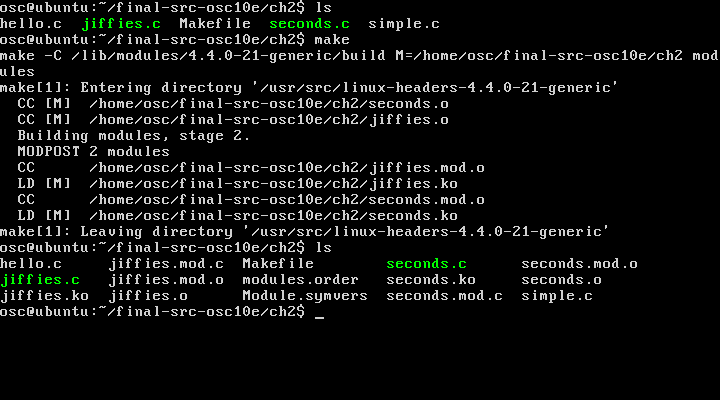
\includegraphics[width=1\textwidth]{make.png}
    \caption{Tạo modules}
\end{figure}
\begin{figure}[h]
    \centering
    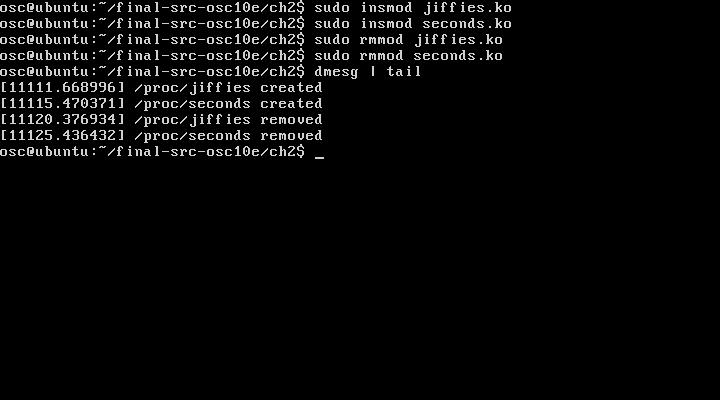
\includegraphics[width=1\textwidth]{load_remove.png}
    \caption{Nạp vào và rời bỏ modules}
\end{figure}
\begin{figure}[h]
    \centering
    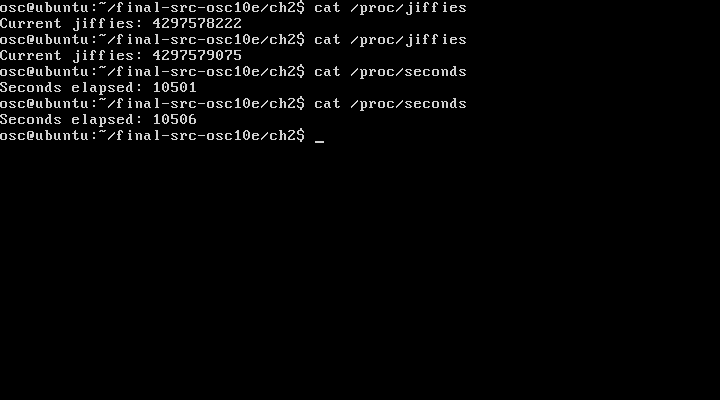
\includegraphics[width=1\textwidth]{results.png}
    \caption{Chạy modules}
\end{figure}
\begin{thebibliography}{9}
    \bibitem{texbook}
    A. Silberschatz, P.B. Galvin, G. Gagne (2018) \emph{Operating System Concepts}, John Wiley \& Sons, Inc, 10th ed.

\end{thebibliography}
\end{document}

